\documentclass[a4paper]{article}

% 文章排版
\usepackage{indentfirst}
\setlength{\parindent}{0em}
\usepackage{autobreak}
\allowdisplaybreaks
\usepackage{parskip}
\usepackage{geometry}
\geometry{top=3cm,bottom=3cm,left=2cm,right=2cm}
\usepackage{anyfontsize}

% 数学物理宏包
\usepackage{amsmath}
\usepackage{physics}
\renewcommand\div\divisionsymbol
\DeclareMathOperator{\diag}{diag}
\DeclareMathOperator{\sgn}{sgn}
\newcommand{\trans}{\text{\textsf{T}}}
\usepackage{tabularray}
\UseTblrLibrary{amsmath}

\usepackage{xcolor}
\usepackage{fontspec}
\setmainfont{STIX Two Text}
\usepackage{unicode-math}
\unimathsetup{mathrm=sym,mathbf=sym,mathsf=sym,bold-style=ISO}
\setmathfont{STIX Two Math}

\usepackage[fontset=none]{ctex}
\setCJKmainfont{FZShuSong-Z01}[BoldFont=Source Han Sans CN,ItalicFont=FZKai-Z03]
\setCJKsansfont{Source Han Sans CN}

% 符号重定义
\AtBeginDocument{
    \let\uglyepsilon\epsilon
    \renewcommand\epsilon\varepsilon
    \let\uglyleq\leq
    \renewcommand\leq\leqslant
    \let\uglygeq\geq
    \renewcommand\geq\geqslant
}

\usepackage{tikz}
\usetikzlibrary{arrows.meta,decorations.pathmorphing,angles,quotes}


% 题目
\title{\textbf{广义相对论（天文方向）\ \ \ \ 作业九}}
\author{国家天文台 张植竣}
\date{2025年11月10日}

\begin{document}

\maketitle

\begin{enumerate}
    \item 银河系中心的黑洞质量大约为$M_{\mathrm{BH}} = 4 \times 10^6\,M_\odot$，地球距离银河系中心大约$8\,\mathrm{kpc}$，那么从地球上看银河系中心黑洞的表观角直径是多少微角秒？作为对比，事件视界望远镜（EHT）在$230\,\mathrm{GHz}$下角分辨率大概是$23\,\upmu\mathrm{as}$。

    \textcolor{blue}{
    将银河系中心黑洞近似视为一个Schwarzschild黑洞，则黑洞视界半径为：
    \[
        R_s = \frac{2GM_{\mathrm{BH}}}{c^2} = \frac{2G}{c^2} \times \qty(4 \times 10^6\,M_\odot) = 1.18 \times 10^{10}\,\mathrm{m}
    \]
    但是对于远处的观测者，黑洞的表观半径并不是视界半径。 \\
    考察光子在Schwarzschild时空中的运动方程（零测地线）：
    \[
        -\qty(1 - \frac{R_s}{r})^{-1} E^2 + \qty(1 - \frac{R_s}{r})^{-1} \qty(\dv{r}{\lambda})^2 + \frac{L^2}{r^2} = 0
    \]
    其中$\lambda$是测地线仿射参数，$E$和$L$分别是光子的“能量”和“角动量”守恒量：
    \[
        E = \qty(1 - \frac{R_s}{r}) \dv{t}{\lambda}, \quad L = r^2 \dv{\phi}{\lambda}
    \]
    定义光子的有效势能为：
    \[
        V_{\mathrm{eff}}(r) = \qty(1 - \frac{R_s}{r}) \frac{L^2}{r^2}
    \]
    引进入射参数$b = \dfrac{L}{E}$，则光子轨道方程可以写成：
    \[
        \qty(\dv{r}{\lambda})^2 = E^2 - V_{\mathrm{eff}}(r)
    \]
    $b$的物理意义如下：以星体中心为原点时，光线在渐近无穷远处近似直线，该直线的延伸线离原点的垂直距离就是$b$（如下图）。
    \begin{figure}
    \centering
    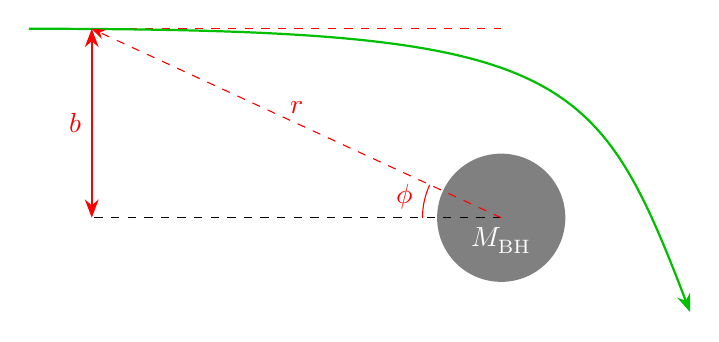
\begin{tikzpicture}[>=Stealth, scale=0.8]
        % 黑洞视界
        \fill [black!50!white] (0,0) circle (1cm);
        \draw [black!50!white,thick] (0,0) circle (1cm);
        \node [below,white] at (0,0) {$M_{\mathrm{BH}}$};
        % 渐近线
        \draw [red,dashed] (-7.5,3) -- (0,3);
        % 散射轨道
        \draw [green!75!black,thick,->] (-7.5,3) .. controls (1,3) and (1.5,2.4) .. (3,-1.5);
        % 入射参数
        \draw [dashed] (0,0) coordinate (O) -- (-6.5,0) coordinate (A);
        \draw [red,<->,thick] (-6.5,0) -- (-6.5,3) coordinate (B) node[midway,left] {$b$};
        \draw [red,dashed,->] (O) -- (B) node[midway,above] {$r$};
        \path (B) -- (O) -- (A) pic [draw,red,angle radius=1cm,"$\phi$",angle eccentricity=1.25] {angle = B--O--A};
    \end{tikzpicture}
    \end{figure} \\
    证明如下：设光子轨道在无穷远处与黑洞中心的垂直距离为$d$。在$\theta = \pi/2$的平面上，引进极坐标$x = r\cos{\phi}$和$y = r\sin{\phi}$，当$r \to \infty$时：
    \[
        b = \abs{\frac{L}{E}} = r^2 \frac{\dv*{\phi}{\lambda}}{\dv*{t}{\lambda}} = r^2 \dv{\phi}{t}
    \]
    在$r \to \infty$时，光子入射角$\phi = d/r$，$\dv*{r}{t} = -1$（这里取光速$c = 1$），则：
    \[
        \dv{\phi}{t} = \dv{\phi}{r} \dv{r}{t} = -\frac{d}{r^2} \times (-1) = \frac{d}{r^2} \implies b = d
    \]
    回到有引力场的情况，考察光子在Schwarzschild时空中的有效势能$V_{\mathrm{eff}}(r)$：
    \[
        \dv{r} V_{\mathrm{eff}}(r) = \dv{r} \qty(\frac{L^2}{r^2} - \frac{L^2 R_s}{r^3}) = \frac{L^2}{r^4} \qty(2r - 3R_s)
    \]
    令$\dfrac{\dd}{\dd{r}} V_{\mathrm{eff}}(r) = 0$，可得极值点$r = 3R_s/2$，此时$V_{\mathrm{eff}}(r)$取得极大值：
    \[
        V_{\mathrm{eff}}^{\max} = V_{\mathrm{eff}}(3R_s/2) = \frac{4 L^2}{27 R_s^2}
    \]
    绘制有效势能曲线如图：
    \begin{figure}[!ht]
    \centering
    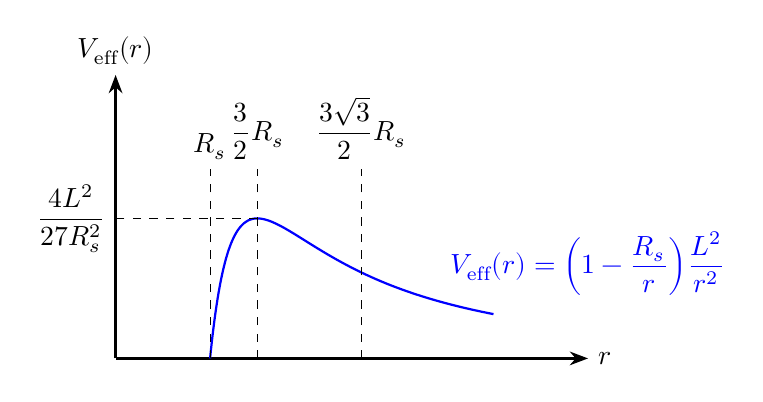
\begin{tikzpicture}[>=Stealth,scale=1.2]
        % 坐标轴
        \draw [->,thick] (0,0) -- (5,0) node[right] {$r$};
        \draw [->,thick] (0,0) -- (0,3) node[above] {$V_{\mathrm{eff}}(r)$};
        % 有效势能曲线
        \draw [thick,blue,domain=1:4,smooth,samples=1000] plot (\x, {10*(1 - 1/\x)/(\x*\x)});
        % 标注
        \node [blue] at (5,1) {$V_{\mathrm{eff}}(r) = \qty(1 - \dfrac{R_s}{r}) \dfrac{L^2}{r^2}$};
        \draw [dashed] (1,0) -- (1,2) node[above] {$R_s$};
        \draw [dashed] (1.5,0) -- (1.5,2) node[above] {$\dfrac{3}{2}R_s$};
        \draw [dashed] (2.5980762,0) -- (2.5980762,2) node[above] {$\dfrac{3\sqrt{3}}{2}R_s$};
        \draw [dashed] (1.5,1.4814815) -- (0,1.4814815) node[left] {$\dfrac{4 L^2}{27 R_s^2}$};
    \end{tikzpicture}
    \end{figure} \\
    因此我们可以得到一个入射参数的临界值$b_{\mathrm{crit}}$：
    \[
        E^2 = \frac{4 L^2}{27 R_s^2} \implies \frac{L^2}{E^2} = \frac{27 R_s^2}{4} \implies b_{\mathrm{crit}} = \frac{L}{E} = \frac{3\sqrt{3}}{2} R_s
    \]
    如下图：入射参数$b < b_{\mathrm{crit}}$时，光子的能量$E^2 < V_{\mathrm{eff}}^{\max}$，则光子会被黑洞捕获；入射参数$b = b_{\mathrm{crit}}$时，光子的能量$E^2 = V_{\mathrm{eff}}^{\max}$，则光子会在$r = 3R_s/2$处做不稳定的圆周运动，形成临界光子球；入射参数$b > b_{\mathrm{crit}}$时，光子的能量$E^2 > V_{\mathrm{eff}}^{\max}$，则光子还能回到无穷远，但轨迹被黑洞偏转（散射）。
    \begin{figure}[!ht]
    \centering
    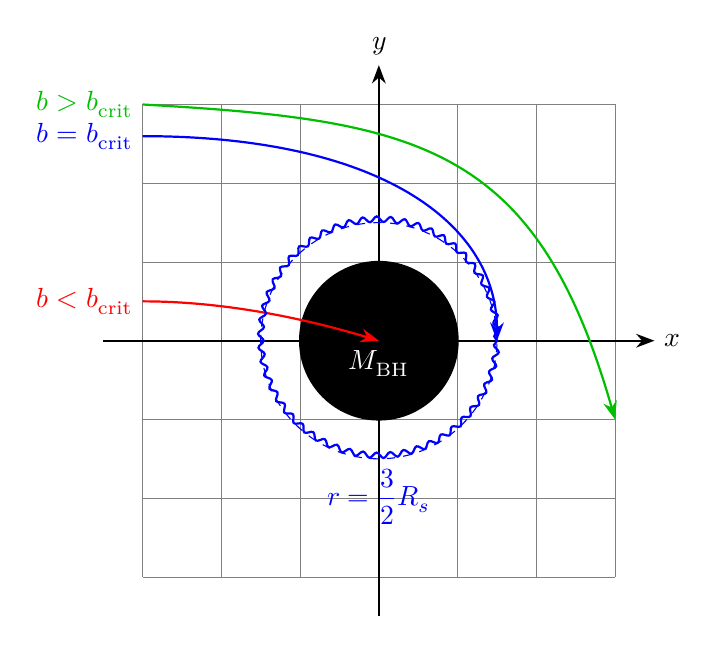
\begin{tikzpicture}[>=Stealth]
        % 坐标轴
        \draw [gray,very thin] (-3,-3) grid (3,3);
        \draw [->,thick] (-3.5,0) -- (3.5,0) node[right] {$x$};
        \draw [->,thick] (0,-3.5) -- (0,3.5) node[above] {$y$};
        % 黑洞视界
        \fill [black] (0,0) circle (1cm);
        \draw [thick] (0,0) circle (1cm);
        \node [below,white] at (0,0) {$M_{\mathrm{BH}}$};
        % 情况1: 被俘获 (b < b_crit)
        \draw [red,thick,->] (-3,0.5) .. controls (-2,0.5) and (-1,0.3) .. (0,0);
        \node [red,left] at (-3,0.5) {$b < b_{\text{crit}}$};
        % 情况2: 临界轨道 (b = b_crit)
        \draw [blue,thick,->] (-3,2.5980762) .. controls (0,2.5980762) and (1.5,1.5) .. (1.5,0);
        \draw [blue,thick,decorate,decoration={snake,amplitude=1pt,segment length=5pt}] (0,0) circle (1.5cm);
        \draw[dashed,blue] (0,0) circle (1.5cm);
        \node[below,blue] at (0,-1.5) {$r = \dfrac{3}{2}R_s$};
        \node [blue,left] at (-3,2.5980762) {$b = b_{\text{crit}}$};
        % 情况3: 被散射 (b > b_crit)
        \node [green!75!black,left] at (-3,3) {$b > b_{\text{crit}}$};
        \draw [green!75!black,thick,->] (-3,3) .. controls (0.5,2.8) and (2,2.5) .. (3,-1);
    \end{tikzpicture}
    \end{figure} \\
    因此，远处的观测者只能看到入射参数$b > b_{\mathrm{crit}}$的光子，即黑洞的表观半径$R_{\mathrm{obs}}$为临界入射参数：
    \[
        R_{\mathrm{obs}} = b_{\mathrm{crit}} = \frac{3\sqrt{3}}{2} R_s \approx 2.6 R_s
    \]
    黑洞的表观直径$d$为表观半径的两倍，即直径为：
    \[
        d = 2R_{\mathrm{obs}} = 3\sqrt{3} R_s = 6.14 \times 10^{10}\,\mathrm{m}
    \]
    表观角直径$\theta$可以通过公式$\theta = \dfrac{d}{D}$计算：
    \[
    \theta = \frac{d}{D} = \frac{6.14 \times 10^{10}\,\mathrm{m}}{8 \times 3.086 \times 10^{19}\,\mathrm{m}} = 2.49 \times 10^{-11}\,\mathrm{rad}
    \]
    将弧度转换为微角秒：（$1\,\mathrm{rad} = \dfrac{180}{\pi} \times 3600\,\mathrm{arcsec} \approx 206265\,\mathrm{arcsec}$）
    \[
        \theta = 5.13 \times 10^{-5}\,\mathrm{arcsec} = 51.3\,\upmu\mathrm{as}
    \]
    因此，银河系中心黑洞的表观角直径约为$51\,\upmu\mathrm{as}$，大于EHT的分辨率$23\,\upmu\mathrm{as}$，因此可以被EHT解析。
    }

\end{enumerate}

\end{document}